Heutzutage müssen insbesondere Unternehmen in der Lage sein, einerseits auf veränderte Marktbedingungen schnell zu reagieren und anderseits stabile und qualitativ hochwertige Systeme zu integrieren und diese gleichzeitig zuverlässig zu unterhalten. \cite{humble_why_2011} 

Anhand des DevOps-Ansatzes wird eine Kultur oder Umgebung etabliert, durch die das Erstellen, Testen und Freigeben von Software schnell, häufig und zuverlässiger erfolgen kann. \cite[S.xxviii]{sharma_devops_2017}

In diesem Zusammenhang sollen Ineffizienzen in den Softwareentwicklungs-, Release- und Betriebsprozessen vermieden werden, die durch die organisatorische Trennung zwischen den Prozessen \cite{lwakatare_devops_2019} oder durch die Fehlkommunikation zwischen den Teammitgliedern\cite{ebert_devops_2016} verursacht werden. 

Die daraus resultierenden Vorteile, die sich bei der Verwendung von DevOps ergeben, reichen von einer schelleren Produktbereitstellung und Problemlösung, bessere Ressourcenauslastung und Automatisierung bishin zu einer stabileren Betriebsumgebung.    

Insgesamt soll das Ziel verfolgt werden, die Softwarebereitstellung kontinuierlich sicherzustellen um so reaktionschnell auf Veränderungen am Markt oder Kundenanforderungen reagieren zu können.

Gründe für die Einführung von DevOps können vielschichtig sein.

Wie bereits beschrieben, ist es für Teams innerhalb der Entwicklung nicht möglich, neue Softwareversionen freizugeben oder Softwareänderungen schnell vorzunehmen, wenn der Betrieb die jeweiligen Funktionen nur langsam bereitstellen kann. \cite[S. 7,8]{sharma_devops_2017} 

Die Folgen sind eine verspätete Bereitstellung von Releases, Fehler in den Releases oder eine fehlende Dokumentation. \cite[S. 24]{alt_innovationsorientiertes_2017}

Hinzu kommen Probleme wie mangelndes Knowhow von Entwicklen über die Betriebnahme der verwendeten System, mangelndes Vertrauen in den Ops-Bereich bei fehlender Stabilität der Systeme, verzögertes Testen an Funktionalitäten oder Verschwendung durch mangelnde Wiederverwendung von Quellcode. \cite{humble_why_2011}  

Vor diesem Hintergrund stehen die Bereiche der Entwicklung und des Betriebs oft im Zielkonflikt "Agilität vs. Stabilität" und sehen sich mit verschiedenen Hindernissen konfrontiert, darunter unbefriedigende Testumgebungen und schlechter Informationsfluss. \cite{lwakatare_devops_2019} \cite[S. 8]{sharma_devops_2017}, \cite{konig_devopswelcome_2019}

Die Abbildung 1 zeigt den chronischen Konflikt, der oftmals innerhalb der IT-Organsisation herrscht, der durch fehlende Interaktion zwischen diesen Bereichen enstehen, die häufig unterschiedliche Ziele und Prozesse verfolgen. \cite[S. 349 - 350]{kim_devops-handbuch_2017}

\begin{figure}[h]
    \centering
    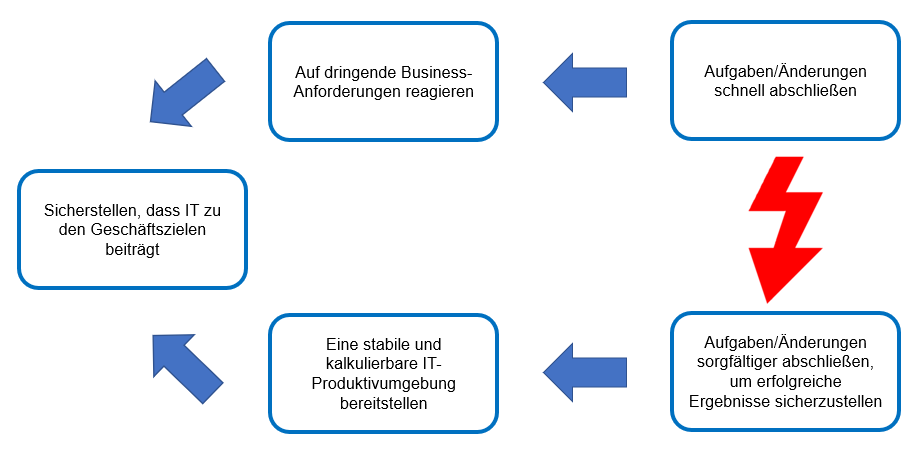
\includegraphics[scale=0.6]{Bilder/Core Conflict Clouds}
    \caption{Zentraler chronischer Konflikt nach Gene Kim \cite[S. 349]{kim_devops-handbuch_2017}}
\end{figure}

Mittels DevOps sollen die Interessen aller an der Bereitstellung von Software Beteiligten ausglichen werden, mit besonderem Schwerpunkt auf Entwicklern, Testern und Betriebspersonal. \cite{humble_why_2011}

Die querschnittlich aufgestellten Teams, lösen sich aus abgegrenzten Organisationseinheiten und Verantwortungsbreichen, aus den sogenannten 'Silos' und treiben gemeinsame Ergebnisse durch eine effektive Zusammenarbeit voran. \cite[S.5]{halstenberg_devops_2020} \cite{sollner_devops_2017}

Generell lässt sich die Werte von DevOps in dem bekannten Akronym CALMS zusammenfassen: Kultur (Culture), Automatisierung (Automation), Schlankheit (Lean), Messung (Measurement) und Teilen (Sharing).  

Der Aspekt der Kultur beinhaltet zunächst die Ausrichtung nach dem Menschen.

Hierbei spielt die Kollaboration als ein funktionsübergreifendes Team und die Orientierung nach Kundenwünschen eine tragende Rolle für eine DevOps-Organisation. \cite[S.5]{halstenberg_devops_2020} 

Die Automatisierung von Entwicklung, Implementierung und Tests ist der Schlüssel zum Erreichen niedriger Vorlaufzeiten und damit zu schnellem Feedback. \cite{humble_why_2011}

'Lean' steht in diesem Zusammenhang für die Vermeidung von Verschwendung jedlicher Ressourcen, Wertgeneration, Transparenz und ganzheitliche Betrachtung und Optimierung von Prozessen.

Der Faktor der Messung orientiert sich an den messbaren Daten, um den Fortschritt eines Unternehmens zu begutachten. 

Die definierten und erhobenen Kennzahlen reichen dabei von den Verfügbarkeiten und den Zeiten für die Fehlerbehebung oder Codeänderungen bis zu den Zeiten für die Anforderungsänderungen. \cite[S. 7]{halstenberg_devops_2020}  

Die letzte Säule beschreibt das Teilen von Informationen, Wissen, Vorgehensweisen und Praktiken innerhalb eines oder zwischen verschiedenen Teams unterschiedlicher Abteilungen. \cite{halstenberg_devops_2020} 

Dabei soll eine Umgebung geschaffen werden, in der gegenseitige Austausch, die Kommunikation und die gemeinsame Nutzung im Vordergrund stehen.

Bei dem gesamten Vorteilen und Mehrwerten, die durch DevOps erreicht werden können, kann DevOps jedoch als kein Nullsummenspiel oder Selbstläufer gesehen werden. \cite{humble_why_2011} 

Der DevOps-Ansatz benötigt zunächst einen kulturellen Wandel, was eine große Herausforderung für viele Unternehmen darstellen kann. 

Standardisierte Herangehensweisen sind von einer Vielzahl von Unternehmen über die Jahre tiefgreifend verankert worden, wodurch Mitarbeiter ihre gewohnten Arbeitsabläufe anpassen müssten. 
 
Dies reicht von der Erlernung neuer Tools, Technologien und Methoden, Aufbau einer Kommunikation für den gegenseitigen Austausch, vollständige Automatisierung, Verschmelzung etablierter Rollen und Zuständigkeiten, Schwierigkeiten bei der Implementierung eines automatisierten Deployment-Prozesses oder die Übernahme neuer Aufgaben und Verantworlichkeiten. \cite{lwakatare_devops_2019}, \cite[S. 594 - 595]{abrahamsson_product-focused_2016}, \cite[S. 43 - 45]{halstenberg_devops_2020}

Da sich die Bedeutung von DevOps in den letzten Jahren verschoben hat und immer wieder neue Tools für DevOps auftauchen, handelt es sich bei DevOps um eine stetige Weiterentwicklung. \cite[S. 595]{abrahamsson_product-focused_2016} 

Daher gibt es keinen Standard fester Praktiken im Zusammenhang mit DevOps, wodurch sich nicht festlegen lässt, welche Praktiken für DevOps eingesetzt werden sollten. 

%Die Trennung zwischen Projekten und Betrieb ist zu einer schwerwiegenden Einschränkung geworden, einerseits für die Fähigkeit von Unternehmen, neue Funktionen schneller auf den Markt zu bringen, andererseits für die der IT, stabile und qualitativ hochwertige Systeme und Dienste zu warten. \cite{humble_why_2011} 

%Ersetzen von Softwareentwicklungsmethode durch Kultur, Bewegung oder Praxis.
%Hinzufügung des Hinweises auf Automatisierung

%In diesem Abschnitt werden die grundsächlichen Merkmale von Devops beschrieben. Zudem werden wesentliche Vorteile beschrieben, durch die die Integration von DevOps möglich sind. Des weiteren wird auf das CALMS-Modell (Culture, Automation, Lean, Measurement und Sharing) eingegangen.

%DevOps gilt nicht als ein Nullsummenspiel, indem die Bereitstellungen häufig und zuverlässig in einer stabilen Produktumgebung erreicht werden, sondern es ist ein Ansatz zur Behebung der genannten Probleme durch Kultur, Automatisierung, Schlankheit, Messung und gemeinsame Nutzung, welches auch als CALMS bekannt ist. \cite{humble_why_2011}